\pagebreak

\section{Supplementary Materials}

\paragraph{Tips for the Supplement.} Please note that the Supplementary Material is not normally read by your examiners. Include material that you might like to include for your own reference, for reference of others beyond your examiners, or as backup to your thesis in case of further discussion.

Here, we use the Supplement to provide further tips on writing your thesis.

\section{Figures}\label{sec:figuresection}

\paragraph{Tips for the Figures.} It is better to create figures in a vector-based format, such as PDF. For plots with very many elements these vector-based graphics can become large and slow to load. In these cases a high-resolution bitmap graphic, such as a png, is preferred. 

Remember to make fonts in figures large enough to be read once the plots are embedded in the report (compare the two plots within Figure~\ref{fig:axis-label-example}). You may need to make multiple versions of the same figure if you plan to use it in your report, poster and presentation.

All figures must be referenced in the main text of the report, in the order that they are referenced.

\begin{figure}[htbp]
    \centering
    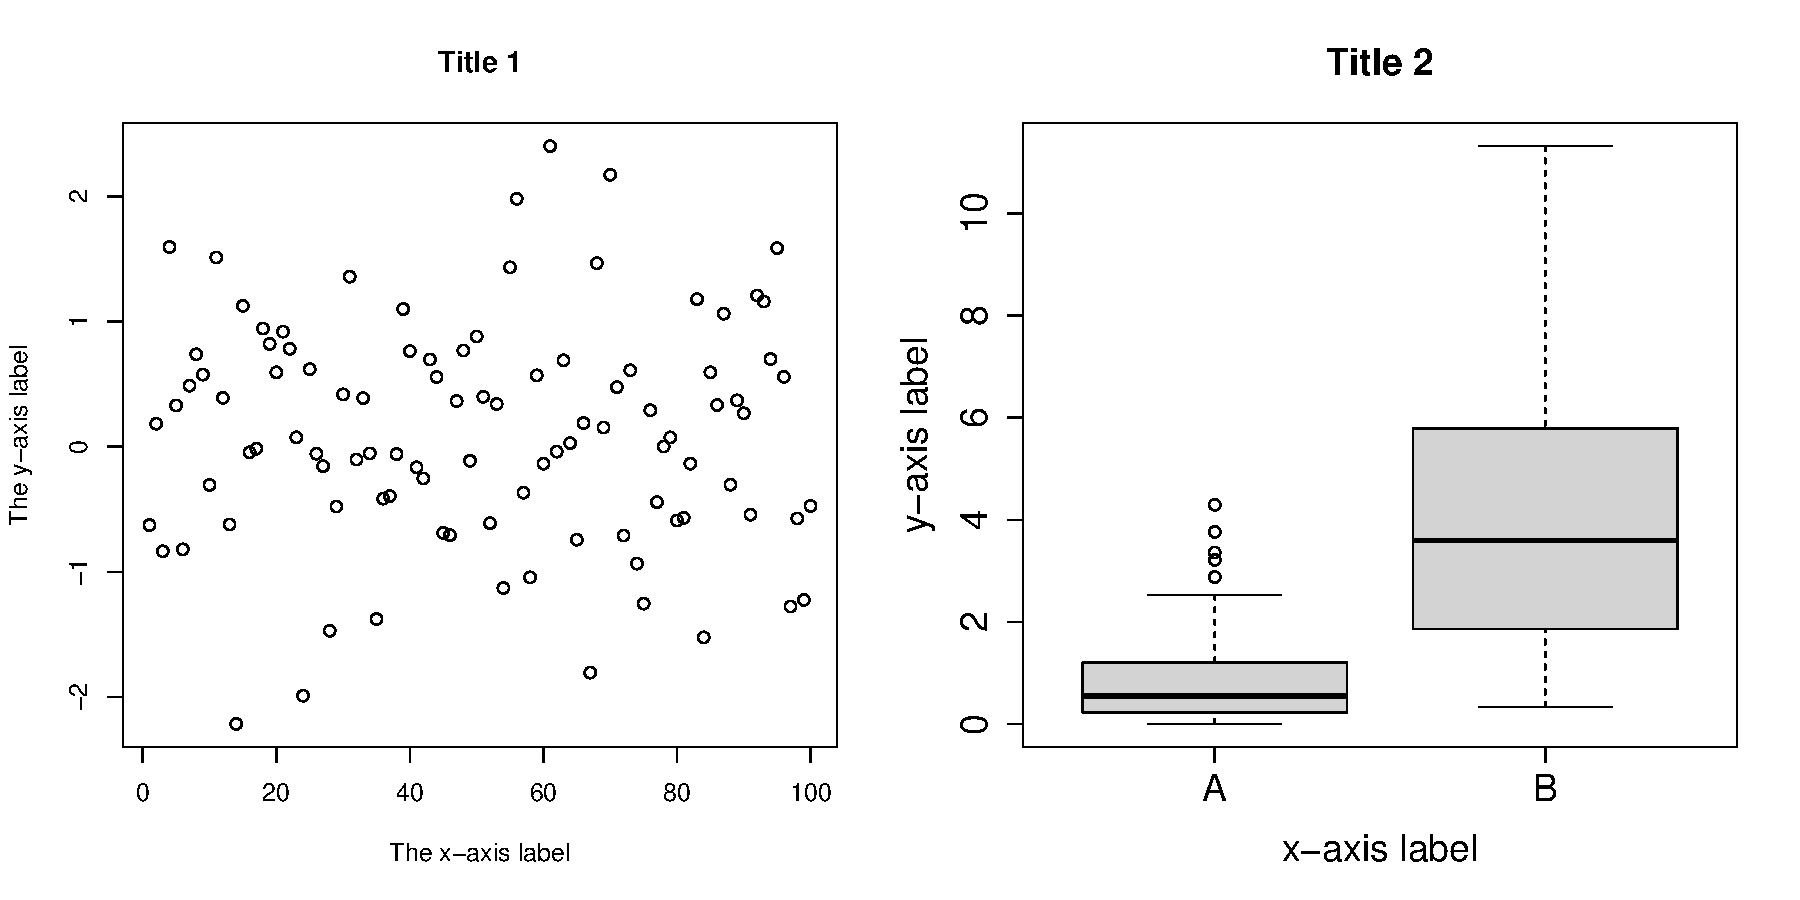
\includegraphics[width=0.9\textwidth]{images/fig1.pdf}
    \caption{An example scatterplot (left) and box plot (right).}
    \label{fig:axis-label-example}
\end{figure}

\section{Tables}\label{sec:tablesection}

\paragraph{Tips for the Tables.} Tables can be a useful way of displaying summary statistics. An example of a simple table is presented as Table~\ref{tab:normal}. All tables must be referenced in the main text of the report, in the order that they are referenced.

\begin{table}[ht]
\centering
\begin{tabular}{rr}
  \hline
    $z$& $\textrm{P}(Z < z)$ \\
  \hline
    1.281& 0.900\\
    1.645& 0.950\\
    1.960& 0.975\\
    2.326& 0.990 \\
    2.576& 0.995 \\
   \hline
\end{tabular}
    \caption{Partial table showing values of $z$ for $\textrm{P}(Z < z)$, 
    where $Z$ has a standard normal distribution.}
    \label{tab:normal}
\end{table}



\section{Referencing sources, sections and items} \label{sec:referencing}

\subsection{Referencing external sources}

You should give attribution to the academic books and articles that you draw from and build upon in your research report. You must give full attribution if and how you used generational AI during your research, referencing its use as outlined in our Guidance to using generational AI on the MSc in Statistics. You should use inline or parenthetical references to these sources. For example, a good book on the bootstrap is \cite{efrontib}, although the idea appeared in an earlier paper \citep{efron1979}.

Note that to make the references appear, you will need to compile the bibtex, otherwise you may just see question marks where the references should be. The small selection of example bibtex references used in this template are provided in the file \texttt{refs.bib}. These should be replaced with your own bibtex entries.
 
\subsection{Referencing elements of your report}

You might also want to cross reference results or claims from another part of your report such a as a section, result or equation. This is done by assigning a \texttt{\textbackslash label\{\}} to the item you wish to cross-reference and then using that label within \texttt{\textbackslash ref\{\}}. For example, Theorem~\ref{thm:variance-mse-relation} is proved in Section~\ref{sec:defnthms}. When referencing displayed mathematics, use \texttt{\textbackslash eqref\{\}}. As an example, see 
Equation~\eqref{eqn:variance-mse-relation}.

\subsubsection{Labelling tables and figures}

It is important that the label command
\texttt{\textbackslash label\{LABELNAME\}} comes \textbf{after} the caption command.
See Table~\ref{tab:normal} and Figure~\ref{fig:axis-label-example} as examples of this.

\subsection{Quoting sources}
If you wish to quote a source, be sure to use quotation marks and cite the
reference. The \texttt{\textbackslash{usequote}} command is useful here:

\usequote{It was the best of times, it was the worst of times, it was the age of wisdom, it was the age of foolishness, it was the epoch of belief, it was the epoch of incredulity, it was the season of Light, it was the season of Darkness, it was the spring of hope, it was the winter of despair, we had everything before us, we had nothing before us, we were all going direct to Heaven, we were all going direct the other way - in short, the period was so far like the present period, that some of its noisiest authorities insisted on its being received, for good or for evil, in the superlative degree of comparison only.} \citep{dickens1859}

\section{Definitions, theorems and examples}
\label{sec:defnthms}

The following environments are supported:
Definition, Theorem, Proof, Proposition, Lemma, Remark, Example.

\begin{definition} \label{defn:variance}
    The \textbf{variance} of a random variable $X$ is defined as
    \begin{equation} \label{eqn:variance-definition}
        \mathrm{Var}(X) = \mathrm{E}[(X - \mathrm{E}[X])^2].
    \end{equation}
\end{definition}

\begin{theorem} \label{thm:variance-mse-relation}
Given a random variable $X$, over all values $a \in \mathbb{R}$, 
\begin{equation}
    \min_{a \in \mathbb{R}} \mathrm{E}[(X - a)^2] 
    = \mathrm{E}[(X - \mathrm{E}[X])^2].
    \label{eqn:variance-mse-relation}
\end{equation}
\end{theorem}

\begin{proof}   
    Starting with the left-hand side of Equation~\eqref{eqn:variance-mse-relation},
\begin{align}
% Example of using \newcommands; see above
\EE{ \inparenth{\X - \consta}^2 } 
&=  \EE{  \inparenth{\X - \EE{\X} + \EE{\X} - \consta}^2 } 
    \nonumber \\
&=  \EE{  \inparenth{ \X - \EE{\X} }^2 } 
    + 2 \EE{ \inparenth{ \X - \EE{\X} } \inparenth{ \EE{\X} - \consta} } +  
  \EE{ \inparenth{ \EE{\X} - \consta}^2  }    
    \nonumber \\
&=  \EE{  \inparenth{ \X - \EE{\X} }^2 } +  \inparenth{ \EE{\X} - \consta}^2
    \nonumber \\
& \geq \EE{  \inparenth{ \X - \EE{\X} }^2 },  
\nonumber 
\end{align}
since $\EE{\X}$ is a real number and $\inparenth{ \EE{\X} - \consta}^2 \geq 0$,
and the third line follows from linearity of expectation:
%
\begin{align}
    \EE{ \inparenth{ \X - \EE{\X} } \inparenth{ \EE{\X} - \consta} }
    =
    \inparenth{ \EE{\X} - \consta} \EE{ \inparenth{ \X - \EE{\X} } }
    =
    \inparenth{ \EE{\X} - \consta}  \inparenth{\EE{ \X} - \EE{\X} } 
    =
    0,
    \nonumber
\end{align}
%
since $\EE{\EE{\X}} = \EE{\X}$, which proves the result.
\end{proof}

\begin{remark}
    This theorem shows that that the minimum of the quantity
    $\mathrm{E}[(X - a)^2]$ is equal to $\mathrm{Var}(X)$.
    In some sense, this makes the variance a natural measure of dispersion if 
    we are taking the metric to be the squared deviation of $X$.
\end{remark}


\begin{lemma}[Stein's Lemma]
    Let $X \sim \mathrm{N}(\mu, \sigma^2)$, and let $g$ be a differentiable 
    function satisfying $\mathrm{E}[|g'(X)|] < \infty$. Then
    \begin{equation}
        \mathrm{E}[g(X)(X-\mu)] = \sigma^2 \mathrm{E}[g'(X)].
        \nonumber
    \end{equation}
\end{lemma}

\begin{proposition}[Popoviciu's inequality]
    Suppose that the random variable $X$ is known to only take values in the 
    bounded range $[a, b]$. Then  
    \begin{align}
        \mathrm{Var}[X] \leq \dfrac{(b-a)^2}{4}.
        \nonumber
    \end{align}
\end{proposition}

\begin{example}
    Suppose $X \sim \mathrm{Bern} (p)$, for some $p \in [0,1]$. Then, 
    since $X \in \{0, 1\}$, $X$ is bounded between $0$ and $1$ and so
    $\mathrm{Var}[X] \leq \tfrac{1}{4}$.
\end{example}

Note that Equations~\eqref{eqn:variance-definition} and \eqref{eqn:variance-mse-relation} are numbered because they are referred to elsewhere in the main text. All other equations are unnumbered. 

Each of these environments may be labelled and referenced as with sections. For example, we might discuss Definition~\ref{defn:variance} or Theorem~\ref{thm:variance-mse-relation} in this paragraph. 
